% ============================================================
%  Chapter 4 — Results
%  Status (M15c, June 2026): §4.1 (tuning window, tasks M7–M9 + M10b
%  depth check), §4.2 (rolling backtest + evaluation suite, M10b–M11),
%  and §4.3 (pool-level accuracy + economic translation, Phase 3
%  M13–M15) all carry real numbers and real artifacts from outputs/.
%  The four Phase-3 placeholders are swapped for F4.1 (fig:poolscatter),
%  T4.2 (tab:poolaccuracy), T5.1 (tab:econerrors), and F5.2
%  (fig:pricerrorbuckets); .tex tables regenerate via
%  dev/model/make_pool_tex.py from the committed M14/M15b JSON. All
%  numbers/tables/figures trace to outputs/{tables,figures}/{loan,pool}_level.
% ============================================================

\chapter{Results}
\label{chap:results}

All results in this chapter are out of sample under the rolling
design of Section~\ref{sec:meth-design} unless explicitly labelled
in-sample.  Negative log-likelihood (NLL) is reported as the mean of
\eqref{eq:nll} over the relevant frozen test rows; lower is better.

\section{Architecture selection and benchmarks on the tuning window}
\label{sec:results-tuning}

Hyperparameter and architecture selection was carried out once, on
the $k{=}2015$ tuning window (training on labels through December
2013, early stopping and selection on validation year 2014), and
frozen thereafter.  The search covered depth
$L\in\{1,3,5,7\}$ $\times$ dropout $\{0, 0.2, 0.5\}$ at zero weight
decay, plus an $\ell_2$ sweep at the five-layer anchor --- a
pruned grid of 14 cells anchored at the five-layer geometry of
\citet{sirignano2021}.

\begin{table}[htbp]\centering\small
\caption[Tuning-window architecture comparison (analogue of
\citealp{sirignano2021} Table 11)]{Tuning-window comparison (the
analogue of Table 11 in \citealp{sirignano2021}): in- and
out-of-sample NLL on the $k{=}2015$ window (dev export) for the
empirical matrix, bucketed matrix, multinomial logit, augmented logit,
neural networks of depth 1/3/5/7, the selected configuration with
dropout, and the eight-network ensemble.  Frequency benchmarks and the
augmented logit carry no in-sample column.}\label{tab:tablea}
% Source: outputs/tables/loan_level/table_a.tex (k=2015 dev export).
% Tabular-only; Unicode sanitized for OT1/pdfLaTeX. Caption+label in chapter4.tex.
\begin{tabular}{lrr}
\toprule
Model & In-sample NLL & Out-of-sample NLL \\
\midrule
Empirical matrix & --- & 0.112661 \\
Bucketed matrix & --- & 0.109247 \\
Logit & 0.141395 & 0.109430 \\
Augmented logit & --- & 0.108843 \\
NN depth 1 (no reg) & 0.136005 & 0.103680 \\
NN depth 3 (no reg) & 0.135114 & 0.104159 \\
NN depth 5 (no reg) & 0.134329 & 0.104299 \\
NN depth 7 (no reg) & 0.134434 & 0.104176 \\
NN-5 + dropout 0.2 & 0.136880 & 0.104845 \\
NN best single ($L{=}3$, dropout 0.2) & 0.133948 & 0.103187 \\
Ensemble $\times 8$ ($L{=}3$, dropout 0.2) & 0.134417 & 0.102741 \\
\bottomrule
\end{tabular}

\end{table}

Three findings from the grid, at dev scale (a stratified
$\sim$3.15-million-row training slice of the window):

\begin{itemize}
\item \textbf{Regularisation moves the optimum deeper.}  Without
  dropout the validation-optimal depth is one hidden layer; with
  dropout $0.2$ it shifts to three --- qualitatively replicating the
  dropout--depth interaction documented by \citet{sirignano2021}.  A
  small $\ell_2$ penalty ($10^{-5}$) partially rescues the five-layer
  network (validation NLL $0.09767 \to 0.09630$) but does not
  overturn the ordering.
\item \textbf{The selected configuration} is depth 3, dropout
  $0.2$: validation NLL $0.09602$, test NLL $0.10319$ on the tuning
  window.  In-sample NLL exceeding out-of-sample in parts of the grid
  is expected here, not inverted overfitting: the expanding training
  window (2000--2013) contains the crisis years while the 2015 test
  year is calm.
\item \textbf{The ensemble helps, with diminishing returns.}  The
  eight-network ensemble at the selected configuration reaches test
  NLL $0.10274$, beating both the average single member ($0.10359$)
  and the best individual member ($0.10307$); the ensemble-size curve
  flattens by roughly five members
  (Figure~\ref{fig:ensemblecurve}).
\end{itemize}

\begin{figure}[htbp]\centering
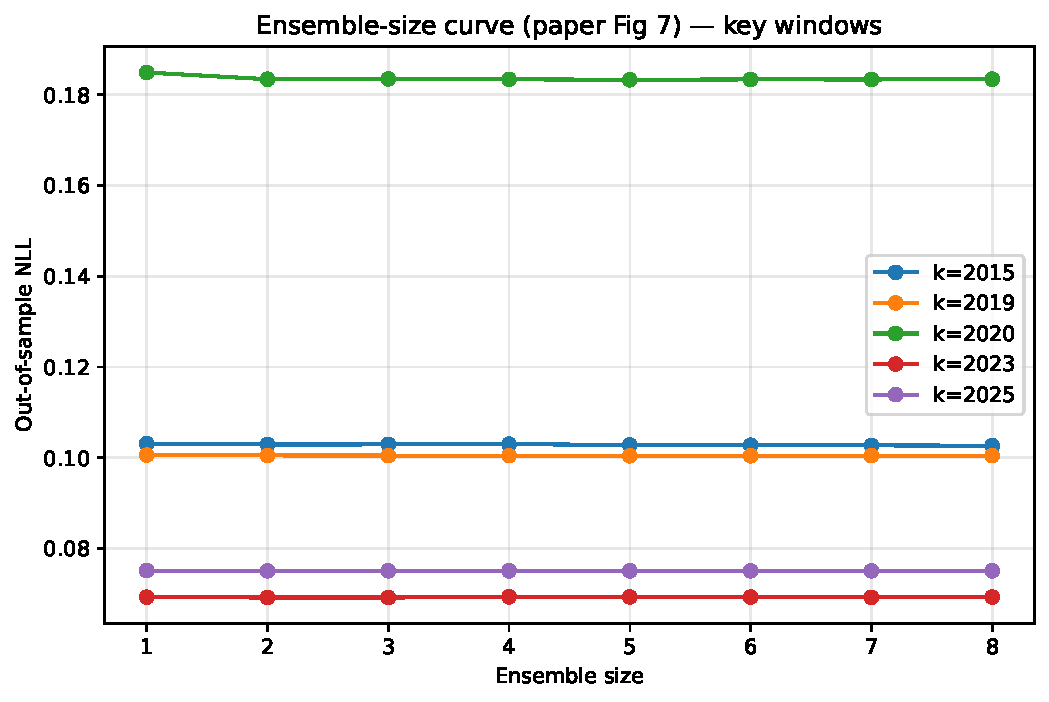
\includegraphics[width=0.8\textwidth]{figs/F_ensemble_size_curve.pdf}
\caption[Out-of-sample NLL versus ensemble size, tuning window]{Out-of-sample
NLL versus number of ensemble members, tuning window (the analogue of
Figure 7 in \citealp{sirignano2021}).}\label{fig:ensemblecurve}
\end{figure}

The multinomial logit baseline was validated against a standard
library implementation (agreement in NLL to within $10^{-3}$ across
the regularisation grid; the loop's embedding-based reimplementation
subsequently matched it to within $10^{-4}$), so the gaps between
logit and network rows in Table~\ref{tab:tablea} are attributable to
architecture alone.

\paragraph{Full-scale depth check.}  Because the grid above was run
at dev scale, the depth choice was re-examined at full scale
($\sim$33.5 million training rows, $10.6\times$ the dev slice) before
the rolling loop was launched: depth 3 and depth 5 were re-fitted on
the full tuning window (with and without the $\ell_2$ rescue).  Depth
3 won robustly on validation (its best validation NLL $0.09572$
against depth 5's $0.09591$), and the frozen configuration for the
loop is depth 3, dropout $0.2$, weight decay $10^{-5}$.  This is a substantive deviation from
\citet{sirignano2021}, whose optimum at population scale was five
layers: on the prime conforming credit box, the optimal network is
\emph{shallower} --- the nonlinearity premium documented in
Section~\ref{sec:data-eda} is real but structurally simpler than in
subprime-heavy private-label data.
%RESULTS-DEPENDENT: revisit wording after M12 (seed variance,
%tuning-window sensitivity on k=2019) to state robustness precisely.

\section{The rolling backtest, 2015--2025}
\label{sec:results-rolling}

The frozen configuration of Section~\ref{sec:results-tuning} --- depth
3, dropout $0.2$, weight decay $10^{-5}$ --- is refitted from scratch
on each of the eleven rolling windows (per-window scaler, embedding
vocabulary, and rate incentive; early stopping on that window's
validation year), alongside a per-window multinomial logit and, on the
five regime-spanning key windows $\{2015, 2019, 2020, 2023, 2025\}$,
an eight-network ensemble.  Every model is scored on the same frozen,
unthinned test slice for its window, so each of the 84.5\,million
pooled test rows is predicted exactly once by a model that never saw
it.

Table~\ref{tab:tableb} is the headline exhibit: out-of-sample NLL by
test year, with the pooled all-years comparison and the by-origin-state
breakdown beneath.  \textbf{The network beats the logit in every one of
the eleven test years} --- calm years, the 2020 COVID forbearance
spike, and the 2022--23 rate shock alike
(Figure~\ref{fig:nllbyyear}).  Pooled over all 84.5\,million test rows,
NLL falls from the $0.111477$ covariate-free empirical floor to
$0.108249$ for the logit and $0.101468$ for the network: the logit
recovers only $2.9\%$ of the distance below the floor while the network
recovers $9.0\%$, so the nonlinearity supplies roughly two-thirds of
the achievable improvement.  The 2020 window is by far the hardest for
every model (NLL ${\approx}\,0.18$--$0.19$, about twice the calm-year
level), reflecting the forbearance-driven distribution shift in the
delinquency codes; the network's relative edge over the logit
nonetheless holds there too.

Because the ensemble was fit only on the five key windows, it is
\emph{not} pooled into the all-years figure --- doing so would compare
it against the logit and network on a different, COVID-weighted set of
rows.  It is read against the network per window instead, in the five
key-year rows of Table~\ref{tab:tableb}: the ensemble's test NLL is at
or below the deployed single network in four of the five (2015, 2019,
2020, 2025) and ties within seed noise on 2023
($+2.2\times10^{-5}$) --- the small variance-reduction effect of
\citeauthor{sirignano2021}'s Figure 7, muted on this cleaner credit
box.

\begin{table}[htbp]\centering\small
\caption[Rolling out-of-sample NLL by test year and origin
state]{Out-of-sample NLL by test year and model, 2015--2025 (top),
with the pooled all-years comparison, and the pooled-NLL breakdown by
origin state (bottom).  Pooled figures are over all eleven windows
(84.5\,M test rows); the eight-network ensemble was fit only on the
five key windows and is therefore reported per year, not pooled --- a
pooled-all-years ensemble figure would mix incomparable row
coverage.}\label{tab:tableb}
% Source: outputs/tables/loan_level/table_b.tex (full export, frozen test slices).
% Tabular-only; Unicode sanitized. The pooled column is restricted to the models
% that exist on all eleven windows (empirical, logit, network): the 8-net ensemble
% was fit only on the five key windows, so a pooled-all-years ensemble figure would
% mix incomparable row coverage and is shown ``---''. The ensemble is compared to
% the network per window in the five key-year rows above. Caption+label in chapter4.tex.
\begin{tabular}{lrrrr}
\toprule
Test year & Empirical matrix & Logit & Best NN & Ensemble $\times 8$ \\
\midrule
2015 & 0.112870 & 0.108246 & 0.103125 & 0.102662 \\
2016 & 0.119296 & 0.116390 & 0.109378 & --- \\
2017 & 0.108116 & 0.105750 & 0.097431 & --- \\
2018 & 0.099608 & 0.098172 & 0.088404 & --- \\
2019 & 0.109673 & 0.106352 & 0.100600 & 0.100479 \\
2020 & 0.193580 & 0.191949 & 0.184869 & 0.183414 \\
2021 & 0.153786 & 0.149628 & 0.141729 & --- \\
2022 & 0.093759 & 0.090422 & 0.085874 & --- \\
2023 & 0.079130 & 0.074943 & 0.069296 & 0.069318 \\
2024 & 0.082829 & 0.079053 & 0.072203 & --- \\
2025 & 0.085575 & 0.082164 & 0.075157 & 0.075095 \\
\midrule
\textbf{Pooled (11 windows)} & 0.111477 & 0.108249 & 0.101468 & --- \\
\bottomrule
\end{tabular}


\vspace{1.5ex}
% Source: outputs/tables/loan_level/table_b.* (pooled NLL by origin state, all 11
% windows, 84.5 M test rows). Ensemble omitted: it exists only on the five key
% windows, so a pooled-all-years ensemble column would mix row coverage.
\begin{tabular}{lrrrr}
\toprule
Origin state & $n$ (rows) & Empirical & Logit & Best NN \\
\midrule
Current   & 82{,}817{,}018 & 0.094731 & 0.091067 & 0.085066 \\
30\,DPD   &    788{,}362 & 1.117058 & 1.147346 & 1.090599 \\
60\,DPD   &    220{,}753 & 1.360988 & 1.387931 & 1.335079 \\
90+\,DPD  &    686{,}244 & 0.575219 & 0.576468 & 0.547682 \\
\bottomrule
\end{tabular}

\end{table}

\begin{figure}[htbp]\centering
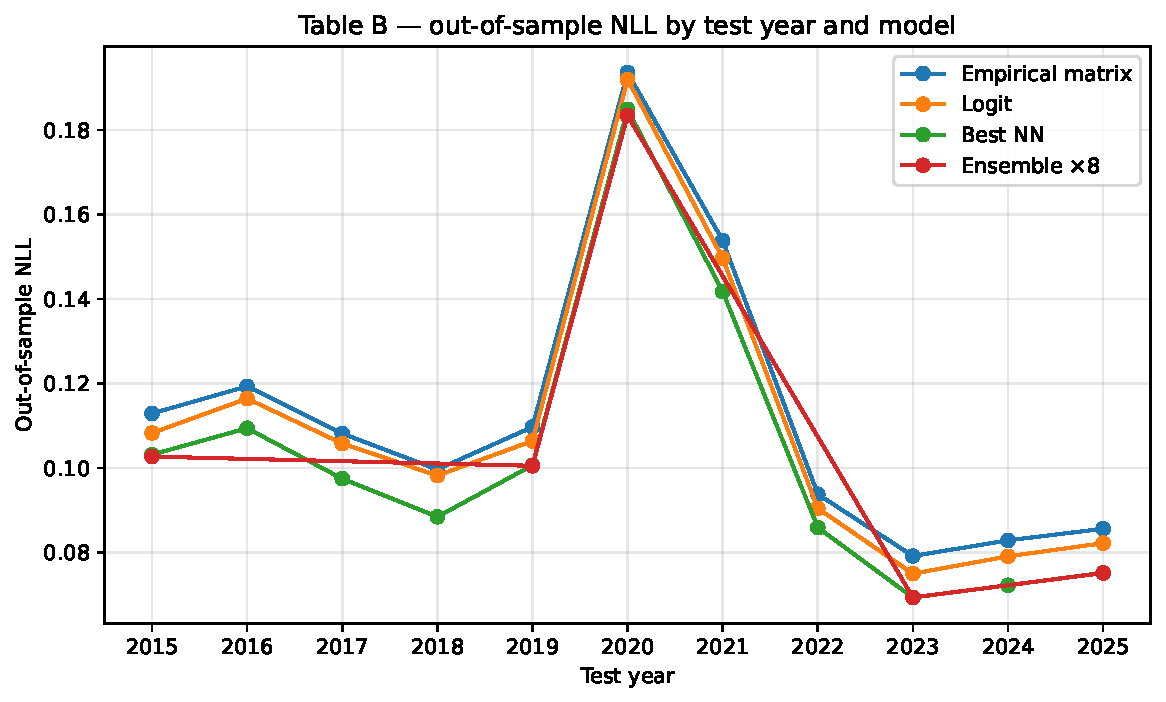
\includegraphics[width=0.85\textwidth]{figs/F_tableB_nll_by_year.pdf}
\caption[Out-of-sample NLL by test year, one line per model]{Out-of-sample
NLL by test year, one line per model: the time series of the value of
nonlinearity.  The ensemble line is drawn only on the five key
windows.}\label{fig:nllbyyear}
\end{figure}

The discrimination gain concentrates exactly where the exploratory
evidence of Section~\ref{sec:data-eda} located the nonlinearity.
Table~\ref{tab:auc} reports one-versus-rest AUC by origin and
destination, pooled over all eleven windows for the two models that
span them.  The network's largest edges are in the prepayment channel
(Current$\to$Prepaid AUC $0.653 \to 0.748$), which combines the
sharpest single-variable nonlinearity with a first-order interaction
with credit, and in the deep-delinquency transitions the logit cannot
even rank (90+\,DPD$\to$Foreclosure $0.482 \to 0.623$, from below
chance to a genuine ranker).  On the five key windows the ensemble's
AUC is at or above the single network's in nearly every cell,
consistent with its marginal NLL gain.

\begin{table}[htbp]\centering\small
\caption[One-versus-rest AUC by transition, all eleven windows
pooled]{One-versus-rest AUC by origin and destination state, pooled
over all eleven windows of test predictions (84.5\,M rows): logit
versus network.  Restricted to the two models fit on every window; the
ensemble (five key windows only) is discussed in the
text.}\label{tab:auc}
% Source: outputs/tables/loan_level/auc.* -- ALL ELEVEN WINDOWS pooled
% (84.5 M test rows), logit vs network. This is the pooled all-years comparison and
% is therefore restricted to the two models that exist on every window. The 8-net
% ensemble (five key windows only) is compared to the network on its matched windows
% in the text. Tabular-only; caption+label in chapter4.tex.
\begin{tabular}{llrrr}
\toprule
Origin & Destination & $n_{+}$ & Logit & Network \\
\midrule
Current  & Current      & 81{,}466{,}577 & 0.6538 & 0.7225 \\
Current  & 30\,DPD      &    438{,}665 & 0.7639 & 0.7684 \\
Current  & Prepaid      &    908{,}017 & 0.6527 & 0.7484 \\
30\,DPD  & Current      &    321{,}129 & 0.6098 & 0.6264 \\
30\,DPD  & 30\,DPD      &    312{,}451 & 0.6152 & 0.6266 \\
30\,DPD  & 60\,DPD      &    141{,}904 & 0.5320 & 0.5322 \\
30\,DPD  & Prepaid      &     11{,}764 & 0.5899 & 0.6659 \\
60\,DPD  & Current      &     33{,}750 & 0.5726 & 0.5883 \\
60\,DPD  & 30\,DPD      &     30{,}105 & 0.5961 & 0.6034 \\
60\,DPD  & 60\,DPD      &     66{,}512 & 0.5590 & 0.5614 \\
60\,DPD  & 90+\,DPD     &     87{,}182 & 0.5481 & 0.5939 \\
60\,DPD  & Prepaid      &      3{,}190 & 0.5559 & 0.6198 \\
90+\,DPD & Current      &     56{,}883 & 0.5890 & 0.6021 \\
90+\,DPD & 30\,DPD      &      7{,}482 & 0.5405 & 0.6294 \\
90+\,DPD & 60\,DPD      &     10{,}519 & 0.5687 & 0.6630 \\
90+\,DPD & 90+\,DPD     &    594{,}879 & 0.5465 & 0.5717 \\
90+\,DPD & Foreclosure  &      4{,}257 & 0.4818 & 0.6233 \\
90+\,DPD & Prepaid      &      8{,}747 & 0.5434 & 0.6257 \\
\bottomrule
\end{tabular}

\end{table}

The aggregate fit is examined two ways.
Figure~\ref{fig:calibration} gives reliability diagrams for the two
dominant Current transitions, pooled and split out for the 2020--21
forbearance years: the network tracks the diagonal markedly better than
the logit, whose miscalibration is worst in the high-hazard upper bins
(the burned-out, deep-in-the-money tail of the prepayment S-curve).
Both models degrade under the 2020--21 shift, but the network remains
the better-calibrated of the two.  Figure~\ref{fig:rateoverlay}
overlays predicted and realised \emph{monthly aggregate} transition
rates over 2015--2025: the network reproduces the level and the timing
of the prepayment waves and the 2022--23 collapse, with the realised
2020 delinquency spike the one place the aggregate prediction lags ---
the expected forbearance-shock miss.

\begin{figure}[htbp]\centering
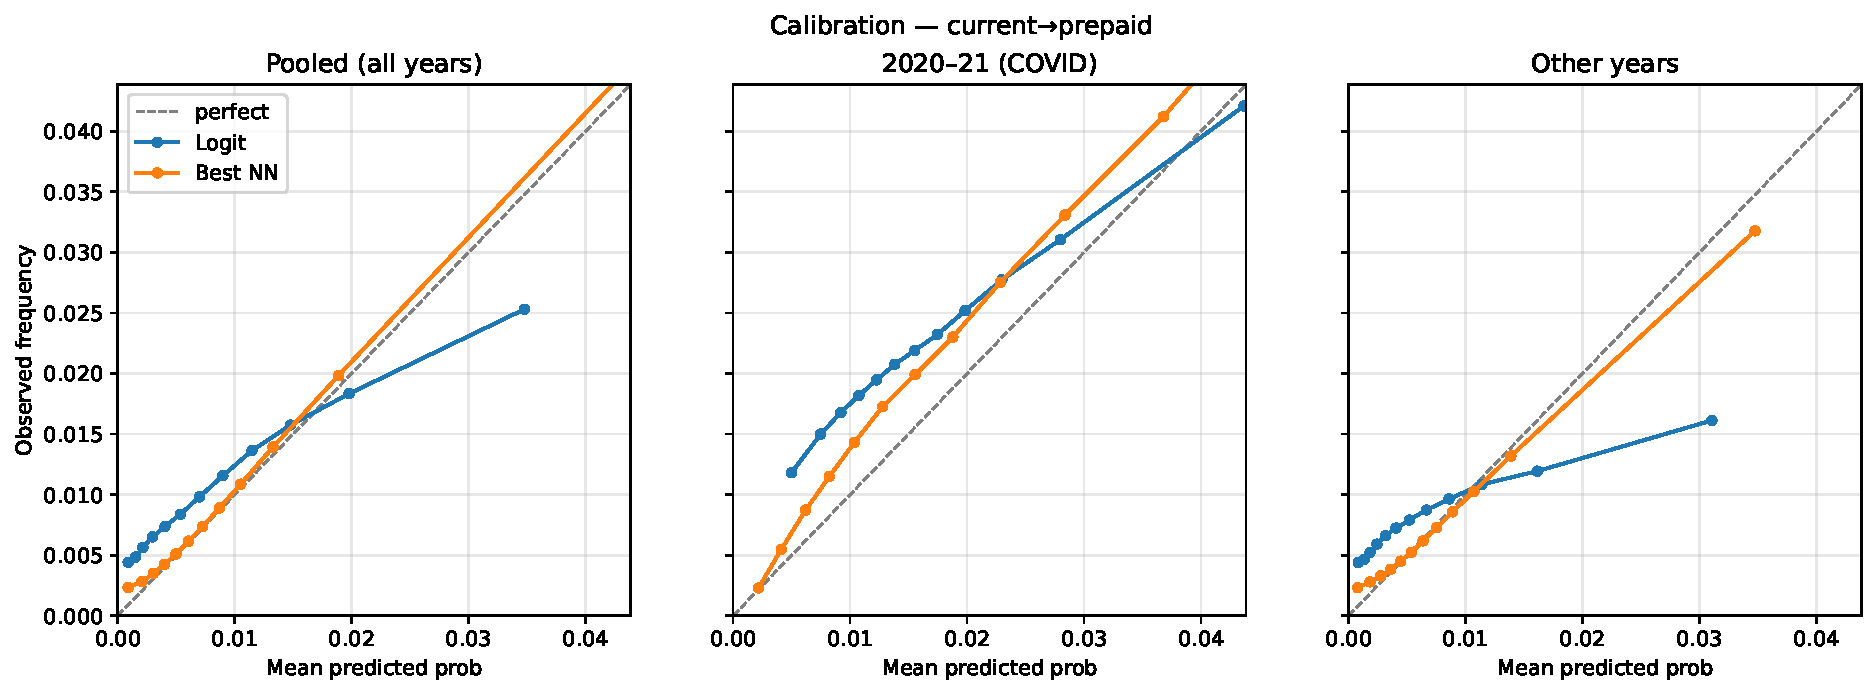
\includegraphics[width=0.49\textwidth]{figs/F_calibration_current_to_prepaid.pdf}\hfill
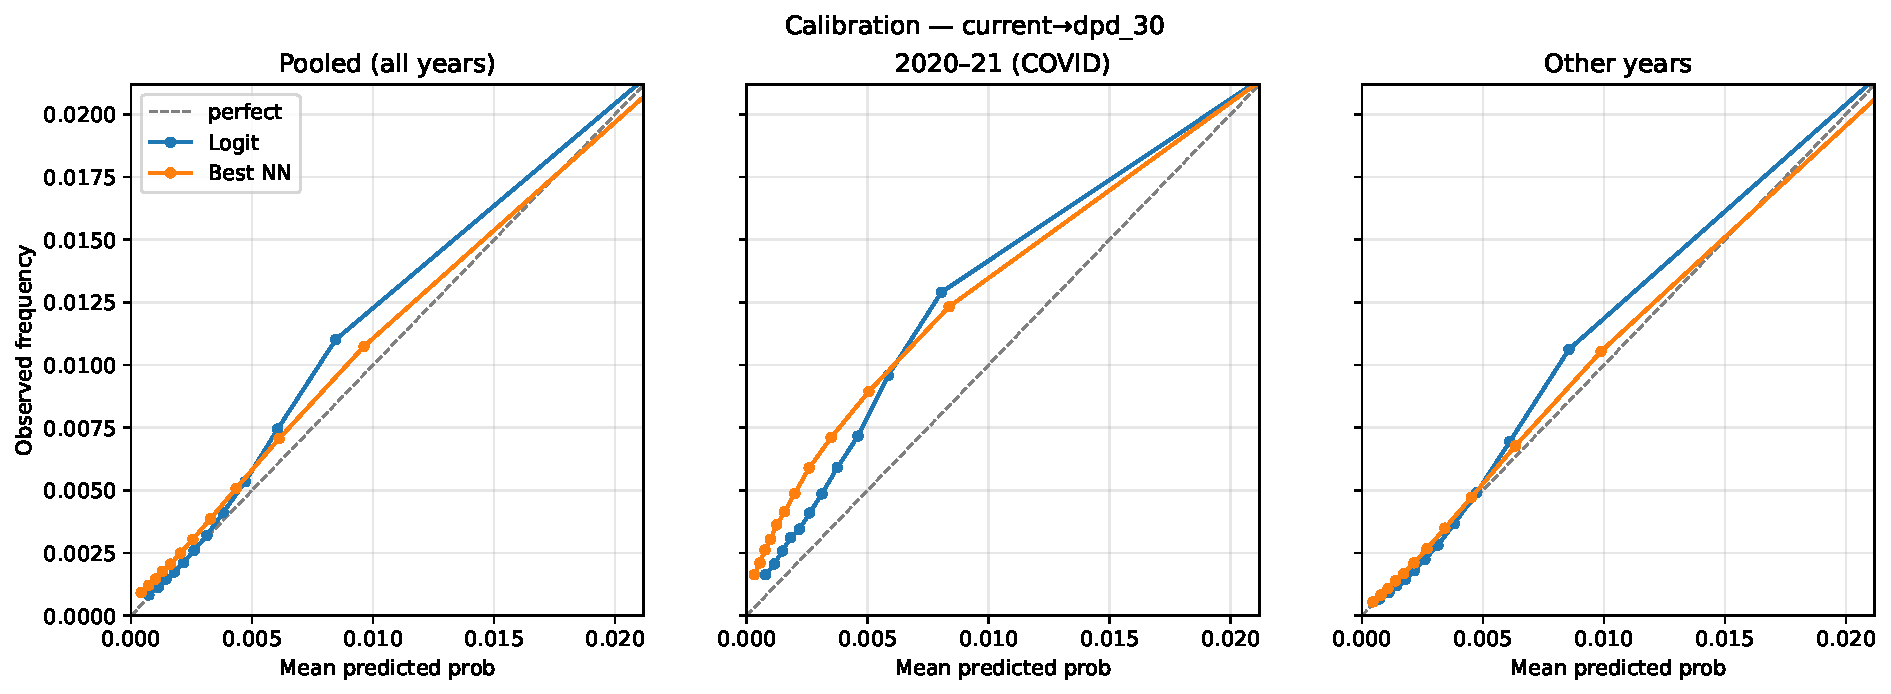
\includegraphics[width=0.49\textwidth]{figs/F_calibration_current_to_dpd_30.pdf}
\caption[Reliability diagrams, Current transitions]{Reliability
diagrams for the Current$\to$Prepaid (left) and Current$\to$30\,DPD
(right) transitions, pooled and for the 2020--21 forbearance years
separately: the network is the better-calibrated of the two
models.}\label{fig:calibration}
\end{figure}

\begin{figure}[htbp]\centering
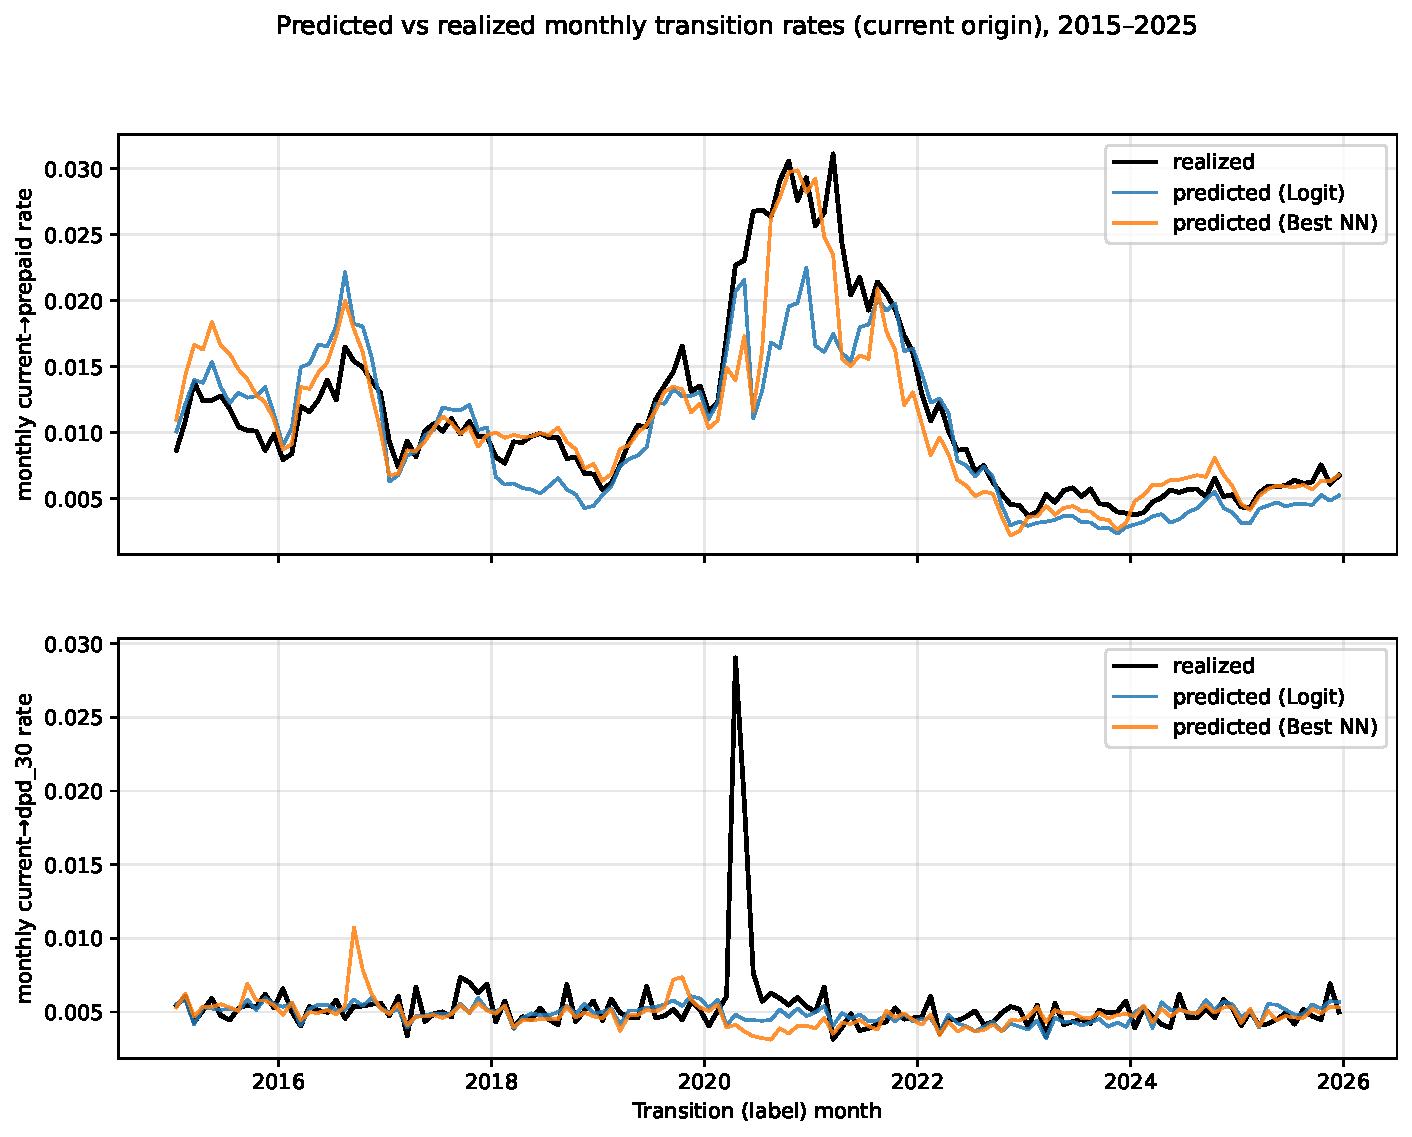
\includegraphics[width=0.85\textwidth]{figs/F_rate_overlay.pdf}
\caption[Predicted versus realised aggregate transition rates]{Predicted
versus realised monthly aggregate Current$\to$Prepaid and
Current$\to$30\,DPD transition rates, 2015--2025.}\label{fig:rateoverlay}
\end{figure}

Robustness exhibits: seed variance of the selected network against the
network--logit gap; stability of the model ranking across the eleven
test years (notably through 2020--21 and 2022--23); re-tuning
sensitivity on the $k{=}2019$ window; and the width sweep at the
selected configuration (Appendix~\ref{app:supplementary}).

\section{Pool-level results and economic translation}
\label{sec:results-pool}

The loan-level models of Section~\ref{sec:results-rolling} are now
aggregated to pools by the roll-forward of
Section~\ref{subsec:meth-pools}: for every loan alive at a window
anchor $t_0{=}\text{Dec}(k{-}1)$, the window-$k$ model's monthly
transition matrices are composed twelve steps forward to a horizon
event probability, and pool counts and speed paths follow from
\eqref{eq:poolcount} and Section~\ref{subsec:meth-econ}.  Only the
deterministic covariates evolve along the chain (loan age, remaining
term, calendar seasonality); the entire macroeconomic block --- rate
incentive, unemployment, house-price growth --- is \emph{frozen at the
anchor}, so every prediction is conditional on the $t_0$ environment.
Five regime-spanning anchors are scored, each with its own frozen
window-$k$ models: Dec2014 (calm), Dec2018 (late cycle), Dec2019
(entering the COVID forbearance shock), Dec2022 (the rate spike), and
Dec2024.

\subsection{Pool-level accuracy and the regime exhibit}

Figure~\ref{fig:poolscatter} is the flagship pool exhibit:
predicted versus realised twelve-month prepayment counts for the 500
random pools at Dec2024, one panel per model.  The improvement in
\emph{level} is stark --- the covariate-free empirical matrix predicts
roughly $2.5\times$ too many prepayments (its flat CPR floor ignores
that the 2024 cohort is deeply out of the money), the logit closes most
of the gap, and the ensemble cloud sits nearest the diagonal (RMSE
$82.9 \to 28.0 \to 11.9$ loans).  The $R^2$ values are all negative
even for the ensemble: random pools are near-homogeneous $1{,}000$-loan
draws, so cross-pool realised variance is tiny and $R^2$ is dominated
by a small level bias --- the random scheme tests \emph{level}
calibration, not cross-pool discrimination, which is why the
discriminating metric is read from the characteristic buckets instead.

Table~\ref{tab:poolaccuracy} gives that characteristic-bucket panel ---
$R^2$ and RMSE by model, outcome, and anchor --- and it is the regime
exhibit promised in Section~\ref{sec:intro-contributions}: a time
series of the value of nonlinearity, not a single verdict.
\textbf{Which model prices a pool best depends on whether the shock
lands in a covariate-captured channel.}  In calm and late-cycle
regimes the covariate models dominate (Dec2014 prepaid $R^2$
$0.58/0.98/0.98$ for empirical/logit/ensemble).  Under the
\emph{rate/prepayment-incentive shock} of 2022--24 --- precisely the
channel the rate-incentive covariates encode --- the empirical matrix
collapses to large negative $R^2$ ($-4.62$ at Dec2022, $-1.46$ at
Dec2024) while the ensemble is strongest ($0.85$, $0.94$; RMSE $415$
against the logit's $991$ at Dec2024).  But under the 2020
\emph{forbearance/credit shock} the ordering \emph{inverts}: at Dec2019
the assumption-free empirical floor is best ($R^2\,0.65$) and the
ensemble is worst ($0.45$), because the ensemble bakes in hardest a
pre-COVID prepayment signal that March 2020 abruptly invalidates.  For
the rare serious-delinquency outcome RMSE is the reliable metric (with
$\sim$16 buckets $R^2$ is unstable across all models), and the ensemble
is the only model with positive $60{+}$\,DPD $R^2$ at the 2022 and 2024
anchors.

\begin{figure}[htbp]\centering
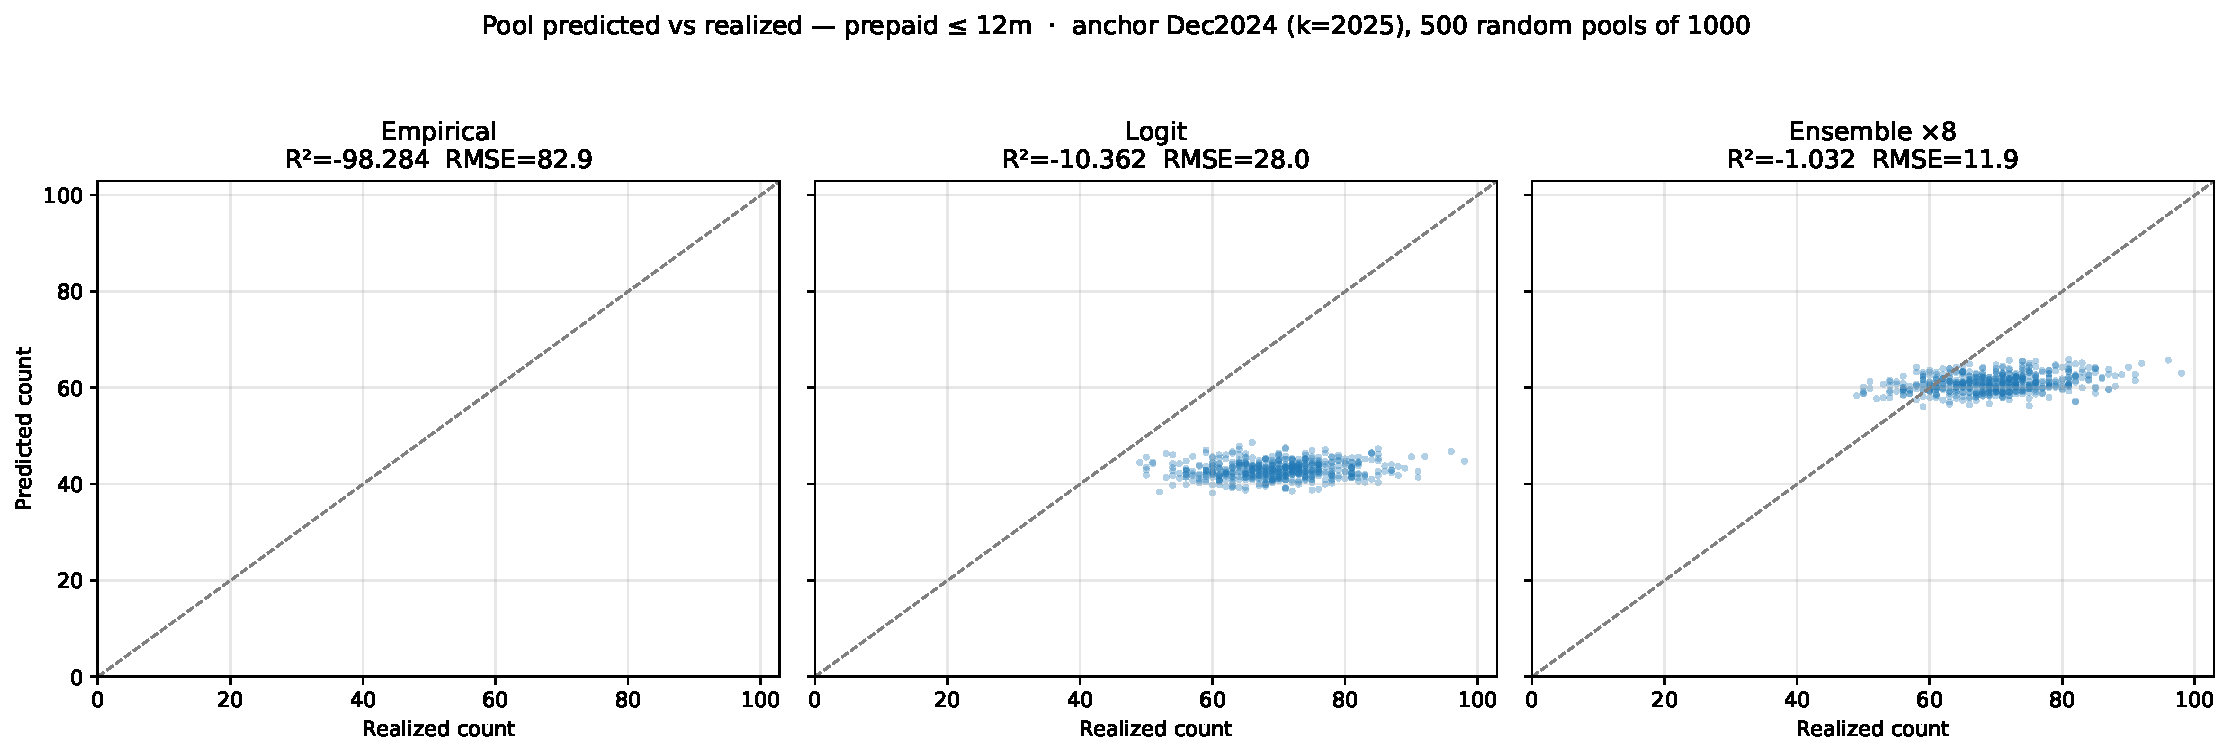
\includegraphics[width=0.95\textwidth]{figs/F4.1_scatter_random_prepaid.pdf}
\caption[Predicted versus realised pool prepayment counts, random
pools]{Predicted versus realised twelve-month prepayment counts, 500
random pools of 1{,}000 loans at the Dec2024 anchor, by model.  The
dashed line is $45^\circ$.  Level calibration improves
empirical\,$\to$\,logit\,$\to$\,ensemble (RMSE $82.9/28.0/11.9$);
$R^2$ is uninformative for homogeneous random pools (see
text).}\label{fig:poolscatter}
\end{figure}

\begin{table}[htbp]\centering\small
\caption[Characteristic-bucket pool accuracy by model, outcome, and
anchor]{Pool-level $R^2$ and RMSE on the characteristic buckets
(credit$\,\times\,$rate$\,\times\,$LTV cells, $\geq2{,}000$ loans each)
by model, outcome, and anchor.  The interpretable cross-pool panel;
random-pool $R^2$ is discussed in the text.  RMSE is in loans.  Shock-type
dependence: covariate models dominate off-COVID and under the rate
shock, but the empirical floor is most robust at the 2020 forbearance
break.}\label{tab:poolaccuracy}
% Source: outputs/tables/pool_level/t_m14_pool_counts.json (M14, full run).
% Characteristic-bucket panel (FICO x orig-rate-quartile x LTV, >=2000 loans/cell): the
% interpretable cross-pool metric. Random-pool R^2 is uninformative by construction
% (homogeneous ~1000-loan draws) and is discussed in text, not tabulated. For the rare
% 60+ DPD outcome read RMSE, not R^2 (>=~16 buckets makes R^2 unstable). Caption in chapter4.tex.
\begin{tabular}{llrrrrrr}
\toprule
 & & \multicolumn{3}{c}{$R^2$} & \multicolumn{3}{c}{RMSE (loans)} \\
\cmidrule(lr){3-5}\cmidrule(lr){6-8}
Outcome & Anchor & Emp. & Logit & Ens. & Emp. & Logit & Ens. \\
\midrule
\multirow{5}{*}{Prepaid} & Dec2014 & 0.575 & 0.980 & 0.981 & 1517 & 328 & 320 \\
 & Dec2018 & 0.744 & 0.607 & 0.791 & 1118 & 1387 & 1011 \\
 & Dec2019 & 0.647 & 0.537 & 0.449 & 3054 & 3500 & 3817 \\
 & Dec2022 & -4.616 & 0.742 & 0.848 & 3303 & 708 & 542 \\
 & Dec2024 & -1.455 & 0.651 & 0.939 & 2627 & 991 & 415 \\
\midrule
\multirow{5}{*}{60+ DPD} & Dec2014 & -4.525 & -0.782 & 0.299 & 449 & 255 & 160 \\
 & Dec2018 & -8.699 & -1.230 & -0.390 & 423 & 203 & 160 \\
 & Dec2019 & -0.165 & -0.467 & -0.464 & 591 & 663 & 663 \\
 & Dec2022 & -17.181 & -0.155 & 0.635 & 514 & 129 & 73 \\
 & Dec2024 & -16.461 & -0.063 & 0.261 & 471 & 116 & 97 \\
\bottomrule
\end{tabular}

\end{table}

\subsection{Economic translation: speed, timing, and price errors}

Restating these count comparisons in valuation units
(Section~\ref{subsec:meth-econ}) sharpens the contribution.
Table~\ref{tab:econerrors} reports mean absolute speed (CPR), timing
(weighted-average life), and price errors on the characteristic
buckets, with the ensemble-versus-logit reduction in the last column;
all errors are model-implied minus realised-speed valuation through the
same engine, so the price column isolates the prepayment forecast.  The
headline is the price row, \textbf{reported per anchor because it
inverts at COVID and a pooled average would conceal that}: the ensemble
cuts the logit's mean absolute price error by $+18\%$ at Dec2014
($0.148\to0.121$ per 100 face), $+25\%$ at Dec2018
($0.560\to0.418$), $+31\%$ at Dec2022 ($0.254\to0.176$), and $+48\%$ at
Dec2024 ($0.233\to0.122$), but by $-1\%$ at the Dec2019 COVID anchor
($0.583\to0.587$) --- the same inversion as the counts, now in price.
The absolute magnitudes are economically modest in aggregate (fractions
of a point per 100 of face), as expected when the discount curve is
fixed and the pools diversify idiosyncratic timing; the action is in
\emph{where} the error concentrates.

Figure~\ref{fig:pricerrorbuckets} maps the signed price error across
credit\,$\times$\,rate cells at the Dec2022 rate-spike anchor, per
model.  The empirical matrix misprices everywhere ($-0.7$ to $-1.2$ per
100, over-predicting prepayment uniformly).  The logit's error is
benign in the low-rate cells but \textbf{concentrates in the
high-incentive top rate quartile} --- $-0.35$ to $-0.61$ per 100, where
its linear-in-incentive form over-fires prepayment on high-coupon loans
whose incentive had in fact collapsed after the 2022 rate rise.  The
ensemble compresses exactly those cells to $-0.15$ to $-0.32$.  This is
the pricing mirror of the prepayment S-curve of
Section~\ref{subsec:data-eda-single}: the linear model breaks where the
hazard is most curved, and that is where dollars of mispricing collect.

\begin{table}[htbp]\centering\small
\caption[Pool CPR, weighted-average-life, and price errors by model and
anchor]{Mean absolute CPR (percentage points), weighted-average-life
(months), and price (per 100 face) error on the characteristic buckets,
by model and anchor, with the ensemble-versus-logit reduction.  Errors
are model-implied minus realised-speed valuation through the same
level-pay engine and discount curve.  The price row is the headline;
reported per anchor because the 2020 anchor
inverts.}\label{tab:econerrors}
% Source: outputs/tables/pool_level/t_m15_econ_errors.json (M15b).
% Characteristic-bucket panel. Each model cell is the mean |error| over the bucket pools;
% errors = model-implied minus realized-SMM valuation through the same level-pay engine
% (identical WAC/WAM/UPB, WAC-25bp curve, so price dispersion isolates the prepay model).
% Last column = ensemble-vs-logit reduction in that row's mean |error| (the price row is the
% headline). Reported per anchor, never pooled (the Dec2019 COVID anchor inverts). Caption in chapter4.tex.
\begin{tabular}{llrrrr}
\toprule
Metric & Anchor & Empirical & Logit & Ensemble & Ens.\,vs\,Logit \\
\midrule
\multirow{5}{*}{\shortstack[l]{Price error\\(per 100 face)}} & Dec2014 & 0.228 & 0.148 & 0.121 & $+18\%$ \\
 & Dec2018 & 0.205 & 0.560 & 0.418 & $+25\%$ \\
 & Dec2019 & 0.552 & 0.583 & 0.587 & $-1\%$ \\
 & Dec2022 & 1.068 & 0.254 & 0.176 & $+31\%$ \\
 & Dec2024 & 0.657 & 0.233 & 0.122 & $+48\%$ \\
\midrule
\multirow{5}{*}{\shortstack[l]{CPR error\\(pp)}} & Dec2014 & 4.30 & 2.34 & 3.28 & $-40\%$ \\
 & Dec2018 & 3.14 & 6.28 & 4.79 & $+24\%$ \\
 & Dec2019 & 17.08 & 16.69 & 17.41 & $-4\%$ \\
 & Dec2022 & 11.80 & 2.69 & 1.56 & $+42\%$ \\
 & Dec2024 & 9.30 & 2.02 & 0.50 & $+75\%$ \\
\midrule
\multirow{5}{*}{\shortstack[l]{WAL error\\(months)}} & Dec2014 & 14.8 & 10.1 & 8.1 & $+20\%$ \\
 & Dec2018 & 13.3 & 38.5 & 28.5 & $+26\%$ \\
 & Dec2019 & 34.0 & 35.7 & 35.8 & $0\%$ \\
 & Dec2022 & 72.0 & 18.9 & 12.9 & $+32\%$ \\
 & Dec2024 & 42.6 & 16.2 & 9.3 & $+43\%$ \\
\bottomrule
\end{tabular}

\end{table}

\begin{figure}[htbp]\centering
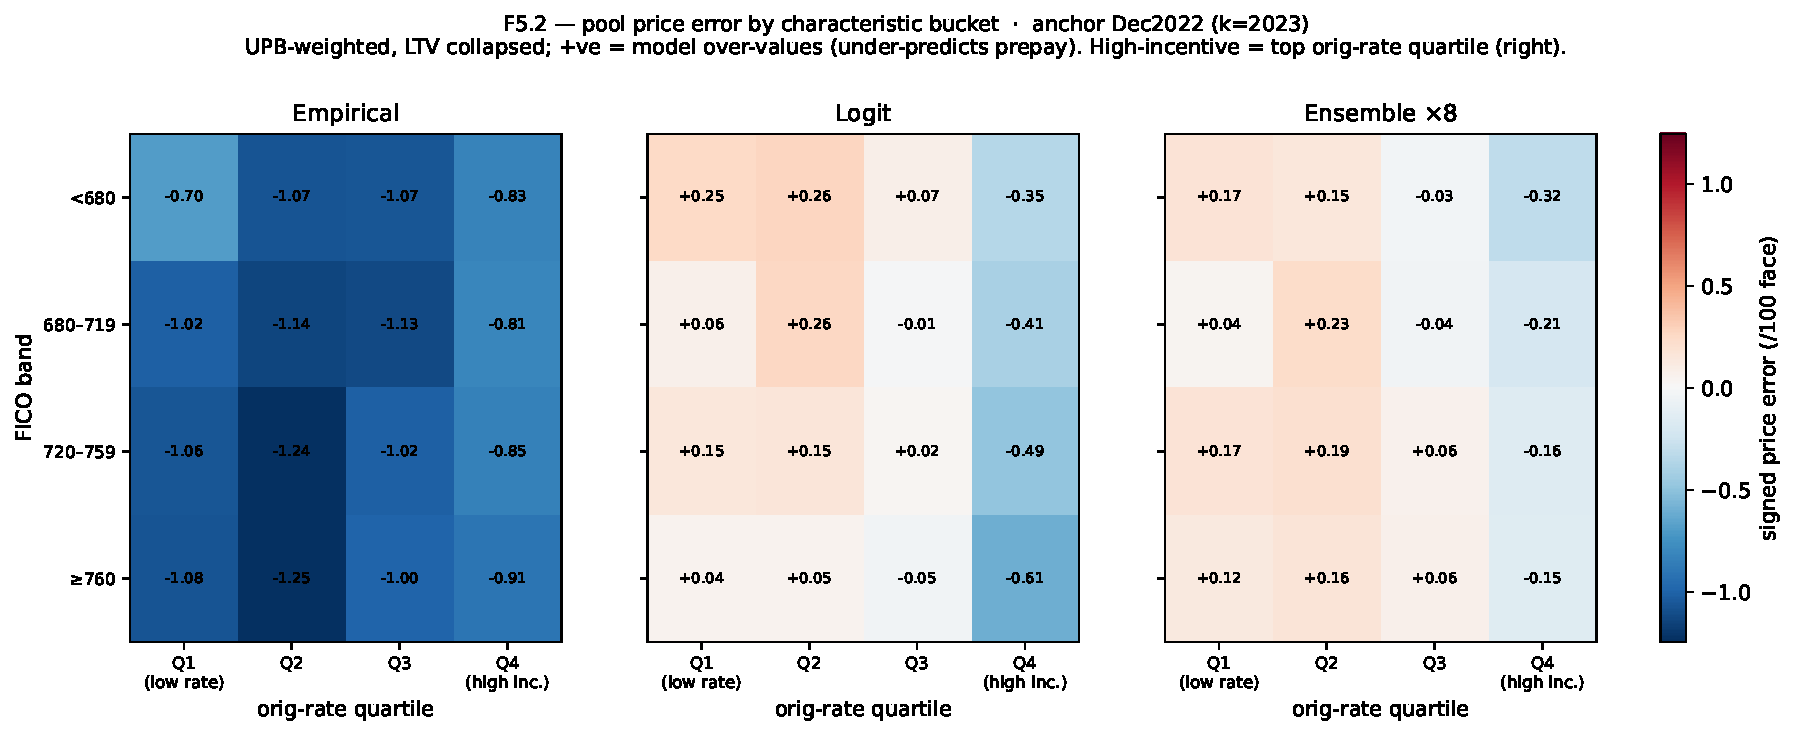
\includegraphics[width=0.95\textwidth]{figs/F5.2_price_error_buckets.pdf}
\caption[Pool price error by characteristic bucket and model]{Signed
price error (per 100 face, UPB-weighted, LTV collapsed) by
credit\,$\times$\,original-rate-quartile cell at the Dec2022 anchor, per
model; positive means the model over-values the pool by under-predicting
prepayment.  The logit's error concentrates in the high-incentive top
rate quartile (right column), which the ensemble
compresses.}\label{fig:pricerrorbuckets}
\end{figure}

\paragraph{Why price is not simply average CPR.}  A pool's price
depends on the \emph{timing} of returned principal --- the full monthly
speed path and hence the weighted-average life --- not on the average
speed alone, which is what makes the cashflow engine more than a
relabelling of CPR.  The two can even rank models differently: at
Dec2014 the logit's mean CPR error is the smaller ($2.34$ against the
ensemble's $3.28$ percentage points), yet the ensemble still prices the
buckets better ($+18\%$ lower price error), because it places its
prepayments at more accurate \emph{months}.  Reassuringly, the engine
is internally coherent --- across all pools and anchors the sign of the
price error agrees with the sign of the weighted-average-life error in
$99.4$--$100\%$ of cases (slower prepayment $\Rightarrow$ longer life
$\Rightarrow$ higher price on these premium pass-throughs).  The
price-versus-CPR sign disagreements occur \emph{only} where the CPR
error is itself negligible (median $0.5$--$1.6$ against $2$--$4.5$
percentage points where they agree): when average speeds nearly match,
timing is what remains, and only the price and life errors can see it.

\paragraph{The frozen-anchor caveat.}  These are
\emph{prepayment-model} valuation errors at a fixed discount curve with
the macroeconomic environment frozen at each anchor, not full
option-adjusted spreads (Section~\ref{subsec:meth-econ}).  The
single regime where this assumption bites hardest is the one it is
designed to expose: at Dec2019 every model under-predicts the realised
$33\%$ CPR by about seventeen percentage points, because all are blind
to the March-2020 rate collapse and refinancing wave that no $t_0$
covariate could anticipate.  Far from a flaw, this is the cleanest
statement of the design's boundary --- it prices the prepayment model,
holding the world fixed --- and it is exactly why the value of
nonlinearity must be read as regime-conditional rather than as a single
headline number.
